%----------------------------
%---------------------------- Document to Create Announcements
%----------------------------

\documentclass[12pt,oneside]{book} 

%----------------------------
%---------------------------- Variables
%----------------------------

\newcommand{\instructor}{Instructor Name}
\newcommand{\labInstructor}{Lab Tech Name} 
\newcommand{\course}{Course} 
\newcommand{\courseCode}{Course Code}
\newcommand{\sect}{000}
\newcommand{\assignment}{Assignment $n$}

%----------------------------
%---------------------------- Packages 
%----------------------------

\usepackage{silence}
\WarningFilter{caption}{}
\usepackage{lipsum}
\usepackage{graphicx}
\usepackage[export]{adjustbox}     
\usepackage{lipsum}
\usepackage{xcolor}
\usepackage{titlesec}
\usepackage{fontawesome5}
\usepackage{enumitem}
\usepackage{booktabs}
\usepackage{fancyhdr}
\usepackage{tikz}
\usepackage[hidelinks]{hyperref}
\usepackage[most]{tcolorbox}
\usepackage{minted}
\usepackage{enumitem}
\usepackage{tabu}
\usepackage{float}
\usepackage[english]{babel}
\usepackage[autostyle, english = american]{csquotes}\MakeOuterQuote{"}
\usepackage[tikz]{bclogo}
\usetikzlibrary{calc,shapes}

%----------------------------
%---------------------------- General Document Formatting
%----------------------------

\usepackage[%
    includefoot,
    includehead,
    left=1.2cm,
    right=1.2cm,
    top=0.7cm,
    bottom=0.7cm]{geometry}

% Interlining = 1.5 and no frikin indent 
\linespread{1.5}
\setlength{\parindent}{0pt}
\setlength{\parskip}{\baselineskip}

% Distance between floats and text  
\setlength{\textfloatsep}{2pt plus 1.0pt minus 2.0pt}
\setlength{\intextsep}{25pt plus 1.0pt minus 2.0pt} 

% Itemize and stuff  

% Sleek Itemize Bullets 
\setlist[itemize]{label=\textcolor{odgreen}{\footnotesize\faChevronRight}}
\setlist[itemize,2]{label=\textcolor{odorange}{\scriptsize\faChevronRight\faChevronRight}} 

% Sleek Enumerate Bullets 
\setlist[enumerate]{label=\textcolor{odmagenta}{\textbf{\small\theenumi.}}}
\setlist[enumerate,2]{label=\textcolor{orange}{\textbf{\small\theenumii.}}}

% Section Headings and stuff
% Customizing section format with a shaded box and a line below, aligned to the right
% Customizing section format, aligned to the right
\titleformat{\section}
{\color{NordBrightCyan}\Large\bfseries\filleft} % aligning title to the right
{}
{0em}
{}
[{\color{NordBrightCyan}\titlerule[1.3pt]}]

\titleformat{\subsection}
{\color{NordGreen}\large\bfseries\filleft} % aligning title to the right
{}
{0em}
{} 
[{\color{NordGreen}\titlerule[0.8pt]}]

\titlespacing{\section}{0pt}{4ex plus 1ex minus .2ex}{3ex plus .2ex}

\titlespacing{\subsection}{0pt}{4ex plus 1ex minus .2ex}{3ex plus .2ex}

\usepackage{unicode-math} % To use the Fira Math font.

\AtBeginDocument{%
    \setmainfont[BoldFont={Fira Sans Bold}]{Fira Sans Book}
    \setsansfont[BoldFont={Fira Sans SemiBold}]{Fira Sans Book}
    \setmonofont[BoldFont={Inconsolata-Bold}, ItalicFont={Inconsolata-Light}]{Inconsolata}
    \setmathfont[BoldFont={Fira Math Bold}]{Fira Math} % Use \symbf{} for bold math
} 

% Captions

\usepackage[skip=0.8pt]{caption} % For better captions

\DeclareCaptionFormat{customFigure}{%
  \textbf{\textcolor{odcyan}{#1#2}}\textcolor{NordBrightestWhite}{#3}}

\DeclareCaptionFormat{customTable}{%
  \textbf{\textcolor{odyellow}{#1#2}}\textcolor{NordBrightestWhite}{#3}}

\captionsetup[figure]{format=customFigure}
\captionsetup[table]{format=customTable}

%----------------------------
%---------------------------- Page Style Definition
%----------------------------

\pagestyle{fancy}
\fancyhf{}
\rhead{{\small\textcolor{odred}{\assignment}}}
\lhead{{\small\textcolor{odorange}{\courseCode}\,\,\textemdash\,\textcolor{odgreen}{\sect}}}
\rfoot{\thepage}
\lfoot{{\small\textcolor{odmagenta}{\instructor}}}
\renewcommand{\headrulewidth}{1pt}
\renewcommand{\footrulewidth}{1pt}
\setlength{\headheight}{15pt}


%----------------------------
%---------------------------- Color Config
%----------------------------

% One-Dark
\definecolor{odbg}{RGB}{40,44,52} % Background 
\definecolor{odfg}{RGB}{171,178,191} % Foreground 
\definecolor{odcomment}{RGB}{92,99,112}
\definecolor{odcyan}{RGB}{86,182,194}
\definecolor{odgreen}{RGB}{152,195,121}
\definecolor{odorange}{RGB}{209,154,102}
\definecolor{odred}{RGB}{224,108,117}
\definecolor{odmagenta}{RGB}{198,120,221}
\definecolor{odblue}{RGB}{97,175,239}
\definecolor{odyellow}{RGB}{229,192,123}

% Nord
\definecolor{NordDarkBlack}{HTML}{2E3440}       % nord0
\definecolor{NordBlack}{HTML}{3B4252}           % nord1
\definecolor{NordMediumBlack}{HTML}{434C5e}     % nord2
\definecolor{NordBrightBlack}{HTML}{4C566A}     % nord3
\definecolor{NordWhite}{HTML}{D8DEE9}           % nord4
\definecolor{NordBrighterWhite}{HTML}{E5E9F0}   % nord5
\definecolor{NordBrightestWhite}{HTML}{ECEFF4}  % nord6
\definecolor{NordCyan}{HTML}{8FBCBB}            % nord7
\definecolor{NordBrightCyan}{HTML}{88C0D0}      % nord8
\definecolor{NordBlue}{HTML}{81A1C1}            % nord9
\definecolor{NordBrightBlue}{HTML}{5E81AC}      % nord10
\definecolor{NordRed}{HTML}{BF616A}             % nord11
\definecolor{NordOrange}{HTML}{D08770}          % nord12
\definecolor{NordYellow}{HTML}{EBCB8B}          % nord13
\definecolor{NordGreen}{HTML}{A3BE8C}           % nord14
\definecolor{NordMagenta}{HTML}{B48EAD}         % nord15

% Code Blocks Background Colors 
\definecolor{draculabg}{RGB}{40,42,54}
\definecolor{materialbg}{HTML}{263238}
\definecolor{onedarkbg}{HTML}{282c34}      

% Set the bg and fg colors
\makeatletter
\newcommand{\globalcolor}[1]{%
    \color{#1}\global\let\default@color\current@color
}
\makeatother

\AtBeginDocument{\globalcolor{NordBrighterWhite}}
\AtBeginDocument{\pagecolor{odbg}}

%----------------------------
%---------------------------- Tcolorboxes
%----------------------------

% Normal Tcolorbox
\newtcolorbox{mybox}[1][]{
    colback=odbg,
    colframe=odblue!60!black,
    colupper=NordBrighterWhite,
    fonttitle=\bfseries,
    title=#1
}

% Modern Tcolorbox
\makeatletter
\newtcolorbox[auto counter]{step}[2][]{%
    enhanced, 
    breakable,
    colback=odbg!95,
    coltext=NordBrighterWhite!85,
    colframe=odgreen!90!black,
    top=0.3cm,
    attach boxed title to top right={yshift=-2pt}, 
    %title={Task \thesection\, -- #2},
    title={\textbf{#2}},
    fonttitle=\large\sffamily,
    coltitle=NordDarkBlack,
    boxed title size=standard,
    boxrule=0pt,
    boxed title style={%
        sharp corners, 
        rounded corners=northeast, 
        colback=tcbcolframe, 
        boxrule=0pt},
    sharp corners=north,
    overlay unbroken={%
        \path[fill=tcbcolback] 
            ([xshift=2pt]title.south west) 
            to[out=180, in=0] ([xshift=-1.5cm]title.west)--
            (title.west-|frame.west) |- 
            ([xshift=2pt]title.south west)--cycle;
        \path[fill=tcbcolframe] (title.south west) 
            to[out=180, in=0] ([xshift=-1.5cm]title.west)--
            (title.west-|frame.west)
            [rounded corners=\kvtcb@arc] |- 
            (title.north-|frame.north) 
            [sharp corners] -| (title.south west);
        \draw[line width=.5mm, rounded corners=\kvtcb@arc, 
            tcbcolframe] 
            (title.north east) rectangle 
            (frame.south west);
    }, 
    overlay first={%
        \path[fill=tcbcolback] 
            ([xshift=2pt]title.south west) 
            to[out=180, in=0] ([xshift=-1.5cm]title.west)--
            (title.west-|frame.west) |- 
            ([xshift=2pt]title.south west)--cycle;
        \path[fill=tcbcolframe] (title.south west) 
            to[out=180, in=0] ([xshift=-1.5cm]title.west)--
            (title.west-|frame.west)
            [rounded corners=\kvtcb@arc] |- 
            (title.north-|frame.north) 
            [sharp corners] -| (title.south west);
        \draw[line width=.5mm, rounded corners=\kvtcb@arc, 
            tcbcolframe] 
            (frame.south west) |- (title.north) -| 
            (frame.south east);
    }, 
    overlay middle={%
        \draw[line width=.5mm, tcbcolframe] 
        (frame.north west)--(frame.south west) 
        (frame.north east)--(frame.south east);
    }, 
    overlay last={%
        \draw[line width=.5mm, rounded corners=\kvtcb@arc, 
            tcbcolframe] 
            (frame.north west) |- (frame.south) -|
            (frame.north east);
    }, 
    #1
}
\makeatother

% Fancy quotes begins %
\makeatletter                 
\NewTColorBox{quotebox}{+O{}+m}{%
    before skip balanced = 0.3cm,
    after skip balanced = 0.4cm,
    enhanced,
    center,
    width=0.9\textwidth,
    sharp corners,
    frame hidden,
    opacityback=.4,
    borderline west={\kvtcb@left@rule}{2pt},
    fontupper=\itshape,
    colback = NordBrightBlue,
    coltext = NordBrightestWhite,
    left=22pt,
    #1,
    overlay={%
        \node[inner sep=0pt,diamond,line width=\kvtcb@left@rule,draw, fill=NordBrightestWhite!70!NordBrightBlue,](framenode) at ($(frame.west)+(2pt+\kvtcb@left@rule/2,0)$) {#2};
  }   
}
\makeatother 


%----------------------------
%---------------------------- Tikz Figures
%----------------------------

% Flowcharts
\usetikzlibrary{calc, shapes.geometric, arrows.meta, positioning}
\tikzset{
  startstop/.style={
    rectangle,
    rounded corners,
    minimum width=3cm,
    minimum height=1cm,
    align = center,
    fill=odgreen,
    draw=NordBrightestWhite,
    line width = 1.1pt,
    text=NordDarkBlack
  },
  io/.style={
    trapezium,
    trapezium left angle=70,
    trapezium right angle=110,
    minimum width=3cm,
    minimum height=1.2cm,
    align = center,
    fill=odred,
    draw=NordBrightestWhite,
    line width = 1.1pt,
    text=NordDarkBlack
  },
  process/.style={
    rectangle,
    minimum width=3cm,
    minimum height=1cm,
    align = center,
    fill=odorange,
    draw=NordBrightestWhite,
    line width = 1.1pt,
    text=NordDarkBlack
  },
  decision/.style={
    diamond,
    minimum width=3cm,
    minimum height=2.5cm,
    align = center,
    fill=NordMagenta,
    draw=NordBrightestWhite,
    line width = 1.1pt,
    text=NordDarkBlack
  },
  predefined/.style={
    rectangle,
    draw=NordBrightestWhite,
    fill=NordBlue,  
    line width=1.1pt,
    text=NordDarkBlack,
    minimum width=5cm,
    minimum height=1cm,
    align = center,
    path picture={
      \draw[line width=1.1pt, NordBrightestWhite] 
      ($(path picture bounding box.north west)+(3mm,0)$) -- ($(path picture bounding box.south west)+(3mm,0)$)
      ($(path picture bounding box.north east)-(3mm,0)$) -- ($(path picture bounding box.south east)-(3mm,0)$);
    }
  },
  comment/.style={
    fill=NordDarkBlack,
    text=NordBrightestWhite,
    minimum width=4cm,
    minimum height=1cm,
    align=center,
    inner sep=4pt,
    path picture={
      \draw[NordBrightestWhite, line width=0.8pt] 
      (path picture bounding box.north west) -- 
      (path picture bounding box.south west) -- 
      (path picture bounding box.south east);
      \draw[NordBrightestWhite, line width=0.8pt] 
      (path picture bounding box.north west) -- 
      (path picture bounding box.north east);
    }
  },
  arrow/.style={
  thick,
  ->,
  >=stealth,
  line width=1.5pt,  % Adjusts the line width
  every join/.style={-stealth, line width=1.5pt},  % Ensures arrow tips on joins are also thicker
  color=NordYellow
  },
  line/.style={
    dashed,
    line width=1pt,  % Adjusts the line width
    color=NordBrightestWhite
  }
}

%----------------
%--------- Minted Environments
%----------------

% PHP Block 
\newminted[php]{php}{
    autogobble, % Ignore Latex indent
    breaklines, % When the line is too long, break it.
    funcnamehighlighting=true, % If true, highlights built-in function names.
    startinline=true, % leading <?php can be omitted.
    xleftmargin=\parindent,
    numbersep=4pt,
    frame=lines,
    framesep=2mm,
    baselinestretch=1.5,
    fontsize=\small,
    bgcolor = draculabg,
    style = nord-darker
}

% PHP in Line
\newmintinline[inlinePHP]{php}{
    xleftmargin=\parindent,
    framesep=2mm,
    funcnamehighlighting=true,
    baselinestretch=1,
    fontsize=\normalsize,
    style = nord-darker
}

% HTML+PHP Block 
\newminted[html]{html+php}{
    autogobble, % Ignore Latex indent
    breaklines, % When the line is too long, break it.
    xleftmargin=\parindent,
    frame=lines,
    framesep=2mm,
    baselinestretch=,
    fontsize=\scriptsize,
    bgcolor = onedarkbg,
    style = one-dark
}

% Bash Block
\newminted[script]{bash}{
    autogobble, 
    mathescape,
    breaklines,
    xleftmargin=\parindent,
    frame=lines,
    framesep=2mm,
    baselinestretch=1.5,
    fontsize=\small,
    bgcolor = draculabg,
    style = dracula
}

% Bash in Line  (CLI in Line)
\newmintinline[inlineCLI]{bash}{
    framesep=2mm,
    fontsize=\small,
    formatcom=\bfseries,
    bgcolor = draculabg,
    style = dracula
}

% CLI Block
\newminted[cli]{shell-session}{
    autogobble, % Ignore Latex indent
    %escapeinside=--, % Escape keywords in comments
    %mathescape,
    breaklines,
    xleftmargin=\parindent,
    frame=lines,
    framesep=2mm,
    baselinestretch=1.5,
    fontsize=\large,
    bgcolor = draculabg,
    style = dracula
}

% SQL Block
\newminted[sql]{mysql}{
    autogobble, % Ignore Latex indent
    breaklines,
    xleftmargin=\parindent,
    numbersep=4pt,
    frame=lines,
    framesep=2mm,
    baselinestretch=1.5,
    fontsize=\small,
    bgcolor = draculabg,
    style = dracula
}

% SQL in Line
\newmintinline[inlineSQL]{mysql}{
    breaklines,
    xleftmargin=\parindent,
    numbersep=4pt,
    frame=lines,
    framesep=2mm,
    baselinestretch=1.5,
    fontsize=\footnotesize,
    bgcolor = draculabg,
    style = dracula
}

% Pseudocode Block
\newminted[pseudo]{text}{
  autogobble, % Ignore Latex indent
  breaklines, % When the line is too long, break it.
  startinline=false, % We'll keep this false for pseudocode
  xleftmargin=\parindent,
  numbersep=4pt,
  frame=lines,
  framesep=2mm,
  baselinestretch=1.5,
  fontsize=\small,
  bgcolor=draculabg,
  style=nord-darker % The style might need adjustments if 'nord-darker' doesn't provide desired aesthetics for pseudocode.
}

% PowerShell Block
\newminted[ps]{powershell}{
    autogobble, % Ignore Latex indent
    %mathescape,
    breaklines,
    xleftmargin=\parindent,
    frame=lines,
    framesep=2mm,
    baselinestretch=1.2,
    fontsize=\small,
    bgcolor = onedarkbg,
    style = one-dark
}

% PowerShell in Line
\newmintinline[ilps]{powershell}{
    framesep=2mm,
    fontsize=\small,
    bgcolor = draculabg,
    style = one-dark
}

% LaTeX in Line
\newmintinline[inlineLATEX]{latex}{
    breaklines,
    xleftmargin=\parindent,
    framesep=2mm,
    baselinestretch=1.5,
    fontsize=\footnotesize,
    bgcolor = draculabg,
    style = dracula
}

%--------------
%--------- Begin document
%--------------

\begin{document} 

%!TEX root = announcement.tex
\begin{titlepage} % Suppresses displaying the page number on the title page and the subsequent page counts as page 1

\center % Center everything on the page


\textsc{\huge {\color{odyellow}St. Clair College} {@} {\color{odblue}Ace Acumen Academy}}\\[1cm] 

\rule{\textwidth}{2pt}

\textsc{\huge {\color{odcyan}Computer Systems Networking}}\\[1cm] % Major heading such as course name

\textsc{\huge {\color{odorange}\course} -- {\color{odgreen}\sect}} % Minor heading such as course title

\rule{\textwidth}{2pt}

\textsc{\huge {\color{odred}\assignment}} % Minor heading such as course title


\,\vfill

\begin{minipage}{0.33\textwidth}
    \begin{flushleft}
        {
            \Large
            \begin{tabular}{@{}c@{}}
            \textit{Instructor}\\[0.5cm]
            {\color{odmagenta}\instructor} % Your name
            \end{tabular}
        }
    \end{flushleft}
\end{minipage}
~
\begin{minipage}{0.33\textwidth}
    \begin{center}
        {
            \Large
            \begin{tabular}{@{}c@{}}
            \textit{Lab Tech/Instructor}\\[0.5cm]
            {\color{odmagenta}\labInstructor} % Your name
            \end{tabular}
        }
    \end{center}
\end{minipage}
~    
\begin{minipage}{0.25\textwidth}
    \begin{flushright}
        {
            \Large
            \begin{tabular}{@{}c@{}}
            \textit{Section(s)}\\[0.5cm]
            {\color{odgreen}\sect}
            \end{tabular}
        }
    \end{flushright}
\end{minipage}


\,\vfill

\today

\end{titlepage}
%!TEX root = ./Assignment.tex

\begin{figure}[h]
    \begin{center}
        \includegraphics[width=0.9\textwidth]{Figures/1}
    \end{center}
\caption{Something}
\end{figure}


\begin{cli}
admin@system:~$ ls -lh | grep "something"
admin@system:~$ ls -lh
admin@system:~$ 
\end{cli}


\begin{quotebox}{\bccrayon}

    Something nice

\end{quotebox}

\begin{itemize}

    \item Stuff

        \begin{itemize}
        
            \item more stuff
            
        \end{itemize}
    
\end{itemize}

\begin{enumerate}

    \item Stuff

        \begin{itemize}
        
            \item More stuff
            
        \end{itemize}

\end{enumerate}

\begin{step}{Date \& Time}

    \underline{There are no classes on Monday, October 9}; thus, it is not possible to conduct the test during the lecture. However, your lab instructor will conduct the \textbf{midterm test during the lab hours between October 10 and 13}. 

    \textbf{Notice:} If I am your lab instructor on Monday, then you will take the midterm during the lab time on Monday October 16.

\end{step}

\begin{step}{Duration}

    You will have a total of \textbf{60 minutes} to \underline{complete and submit} the test.

\end{step}

\begin{step}{Format}

    \begin{itemize}

        \item The test will be a combination of MCQ and Short Answer Questions

        \begin{itemize}
        
        \item \textbf{15 MCQs} [50\%] 

        \item \textbf{5 short answer questions} [50\%] 
            
        \end{itemize}
        
        \item You can have access to your \textbf{Linux Server, \underline{not the desktop version.}}

        \item You will take the test through \textbf{Microsoft Forms} using the school's computers.

    \end{itemize}
    
\end{step}

\begin{step}{Contents}
    
    The test will \underline{comprehensively} evaluate knowledge from \textbf{weeks 1 to 5}.

\end{step}


\begin{step}{Rules}
    
    \begin{itemize}

        \item \textbf{Absolutely no communication during the test.}

        \item \textbf{Cheating will result in a grade of zero in the test and an Academic Misconduct Form.}

    \end{itemize}

\end{step}

\begin{step}[colframe=odblue]{Sample MCQ}
    
\textbf{Question:} Which of the following Linux distribution is best suited for servers?

        \begin{itemize}
            \item Ubuntu Desktop
            \item CentOS
            \item Kali Linux
            \item Manjaro
        \end{itemize}

\textbf{Answer: CentOS}

\end{step}

\begin{step}[colframe=odblue]{Sample Short Answer Question}
    
\textbf{Question:} See my prompt below. I have a file named \inlineCLI{file1} in my home directory. Type the command to append the string "I am acing this test" to \inlineCLI{file1} without changing the current working directory.

\begin{cli}
# My prompt is as below
admin@system:/usr$ 
\end{cli}

\textbf{Possible Answer:} \inlineCLI{echo "I am acing this test" >> /home/admin/file1}\\

\textbf{Possible Incorrect Answer:} \inlineCLI{echo "I am acing this test" >> file1}\\

\textbf{Explanation:} The promt lets me know that my current working directory is \inlineCLI{/usr}. Thus, if I want to append a string to \inlineCLI{file1}, I need to specify the file's absolute path after stdout redirection.

\end{step} 

\begin{center}

\resizebox{0.9\linewidth}{!}{%

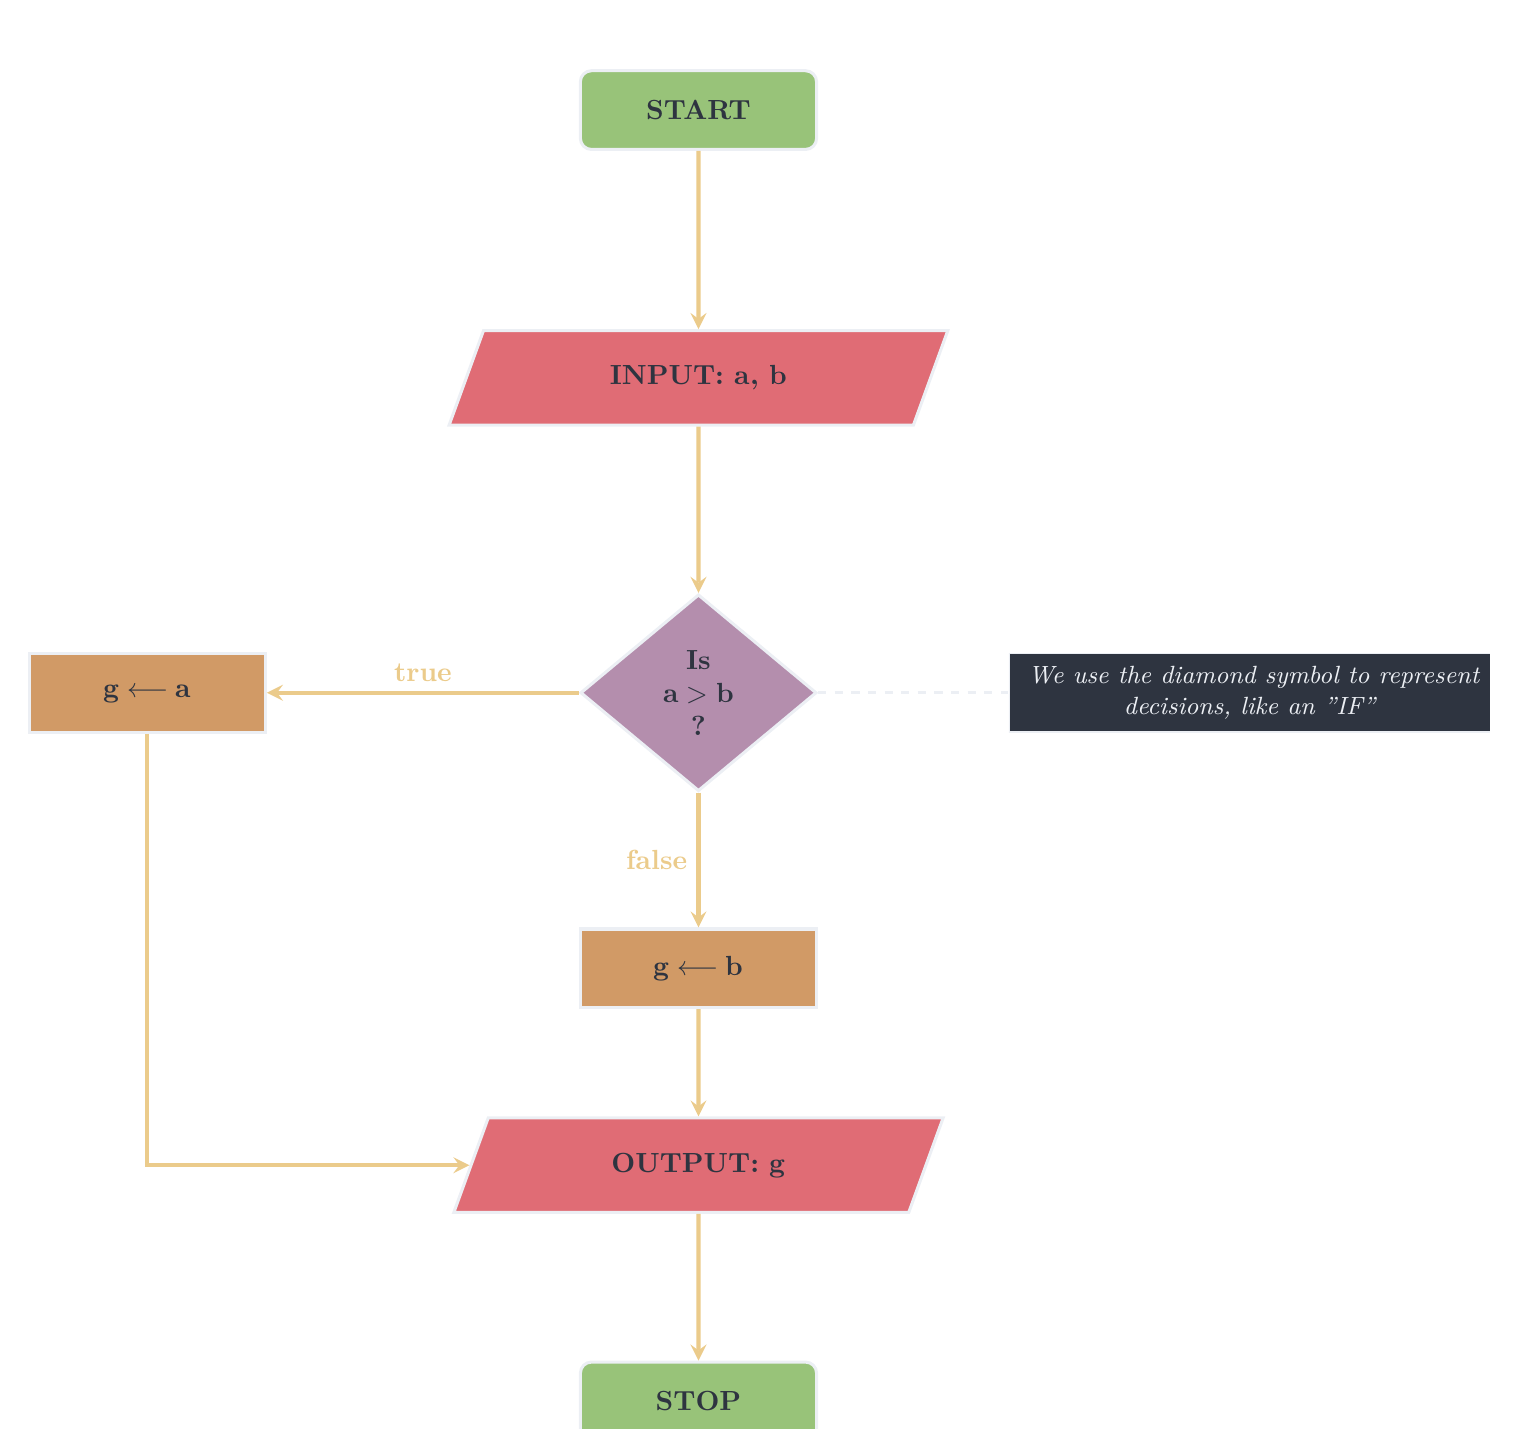
\begin{tikzpicture}[node distance = 2cm, every node/.style={font=\bfseries}]

  \node (start) [startstop] {START};
  \node (input) [io, below of=start, yshift=-1.4cm] {INPUT: $\symbf{a}$, $\symbf{b}$};
  \node (decision) [decision, below of=input, yshift=-2cm] {Is\\ $\symbf{a > b}$\\?};
  \node (comment) [comment, right of=decision, xshift=5cm, font=\small\itshape] {\,\,We use the diamond symbol to represent\\ decisions, like an "IF"};
  \node (truebranch) [process, left of=decision, xshift=-5cm] {$\symbf{g \longleftarrow a}$};
  \node (falsebranch) [process, below of=decision, yshift=-1.5cm] {$\symbf{g \longleftarrow b}$};
  \node (output) [io, below of=falsebranch, yshift=-0.5cm] {OUTPUT: $\symbf{g}$};
  \node (stop) [startstop, below of=output, yshift=-1cm] {STOP};
  
  % Connect nodes with arrows
  \draw [arrow] (start) -- (input);
  \draw [arrow] (input) -- (decision);
  \draw [line] (decision) -- (comment);
  \draw [arrow] (decision) -- node[anchor=south] {true} (truebranch);
  \draw [arrow] (decision) -- node[anchor=east] {false} (falsebranch);
  \draw [arrow] (truebranch) |- (output);
  \draw [arrow] (falsebranch) -- (output);
  \draw [arrow] (output) -- (stop);

\end{tikzpicture}

}

\end{center}

\lipsum[1-7]

\begin{step}{Instructions \& Specs}

    \textbf{Instructions:}

    \begin{enumerate}

        \item Create a new Word document. 

        \item Include a cover page with relevant information:

            \begin{itemize}
            
                \item Your name
                
                \item Your student ID
                
                \item Your section
                
                \item The course name, i.e., Introduction to Programming with PowerShell.
                
            \end{itemize}

        \item Take screenshots where specified in this lab and paste them into your Word document \textcolor{NordOrange}{\textbf{in the correct order}}. 

        \item Answer \textcolor{NordOrange}{\textbf{all}} the questions (if any.)

        \item Save the Word file as \textcolor{NordYellow}{\texttt{Assignment\_8\_FirstName\_LastName.docx}}. Also, save your code as \textcolor{NordYellow}{\texttt{Assignment\_8\_FirstName\_LastName.txt}} file.

        \item Upload your word and .txt files to the lab on Teams.
            
    \end{enumerate}

    \textbf{Specifications:}

    \begin{enumerate}

        \item Ensure each figure shows all the required information, including information that certifies the authenticity of your work, for example:

            \begin{itemize}
            
            \item \underline{Comments in your code} 
            
            \item \underline{Unique Solutions}
            
            \item \underline{Your name and ID in the places I specify}
                
            \end{itemize}
            
        \item Use unique formatting so your work is easily distinguishable from others, but remember that \textbf{\textcolor{NordOrange}{your document must look professional};} please refrain from using fluorescent colours and extravagant fonts. 

        \item Total number of screenshots and questions: \textbf{\textcolor{NordRed}{1}}.

    \end{enumerate}
    
\end{step}

\section{Procedure}

\subsection{Problems}

\begin{step}[colframe=odgreen]{Problem}

    Create a PowerShell script that does the following:

    \begin{itemize}
    
        \item Use a while loop to populate an array with the user's input. The elements of the array should be positive integers.

        \item Create a function that calculates the \href{https://en.wikipedia.org/wiki/Geometric_mean}{\color{NordGreen}{\underline{Geometric Mean}}}  of the numbers above.

        \item The function should receive pipeline input from the array you created above. 

        \item Ensure to include parameter validation so the elements of the array are not larger than 10000.

        \item Ensure the user's values do not produce an indefinite result, i.e., calculate an even root of a negative number.
        
    \end{itemize}

\end{step}



%--------------
%--------- End document
%--------------

\end{document}  